\chapter{Slicer}\label{slicer}

This module has the duty to turn the encapsulator output into user chosen chunks of bits.
This module is necessary because the ATB interface has a specific sized data bus on which data 
has to travel.

The \textit{slicer} reads the outputs of the encapsulator module: header, timestamp and payload.
Then, they are all put in a single array and starting from the least significant byte, they are 
output one slice per cycle, along with the number of valid bits inside each slice.
The output of this module is connected to a fifo, and when it is full, the module stops 
outputting slices and waiting for the fifo to have a free entry.
The number of valid bytes per slice is necessary for the ATB interface, as required by the AMBA 
ATB specification.

On instantiation, the \textit{SLICE\_LEN} parameter can be selected to make it compliant with the 
data bus size used by the ATB interface.

\begin{figure}[H]
    \centering
    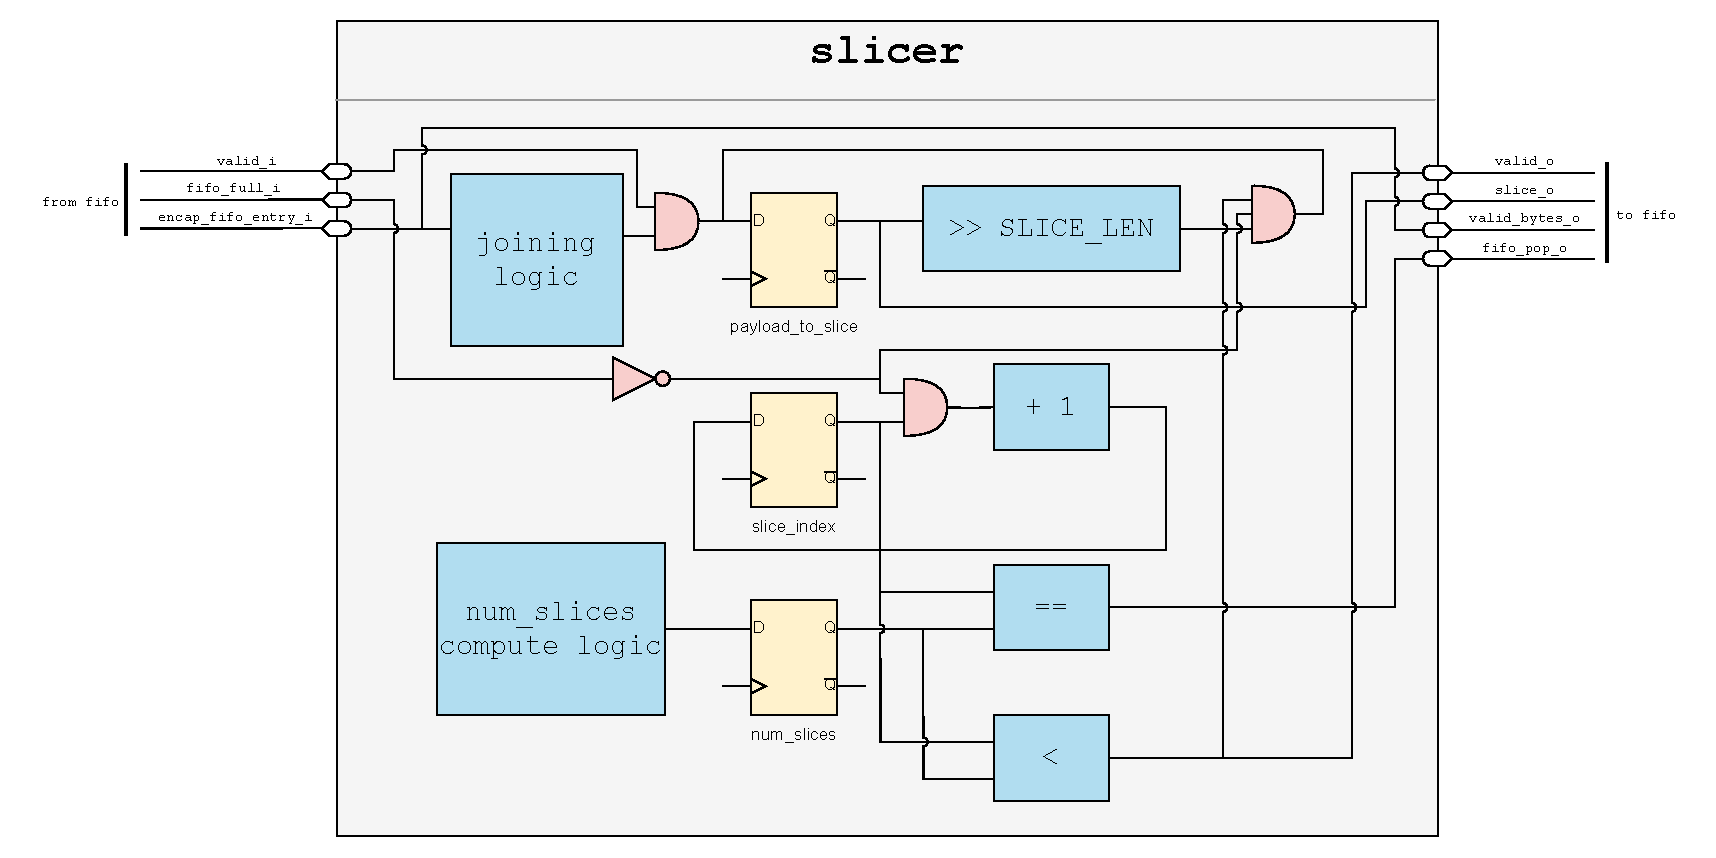
\includegraphics[width=1\textwidth]{img/slicer.pdf}
    \caption{Slicer module internal architecture}
    \label{fig:slicer_architecture}
\end{figure}